\documentclass{article}

\usepackage{url} 

\usepackage{pdfpages}
\usepackage{lastpage}
\usepackage{fancyhdr}
\usepackage{ngerman}




\usepackage{floatrow}
\usepackage[tableposition=top]{caption}
\floatsetup[table]{capposition=top}

\usepackage{amsmath, amssymb}

\usepackage[utf8]{inputenc}


\usepackage[numbib]{tocbibind}

%Gummi|065|=)
\title{Quincke-Kundt}
\author{Johannes Winkler}
\date{}


\newcommand\twodigits[1]{%
   \ifnum#1<10 0#1\else #1\fi
}



\lhead{Quincke-Kundt}
\rhead{\today\\Johannes Winkler}
\cfoot{\twodigits{\thepage}~/ \pageref{LastPage}}

\begin{document}

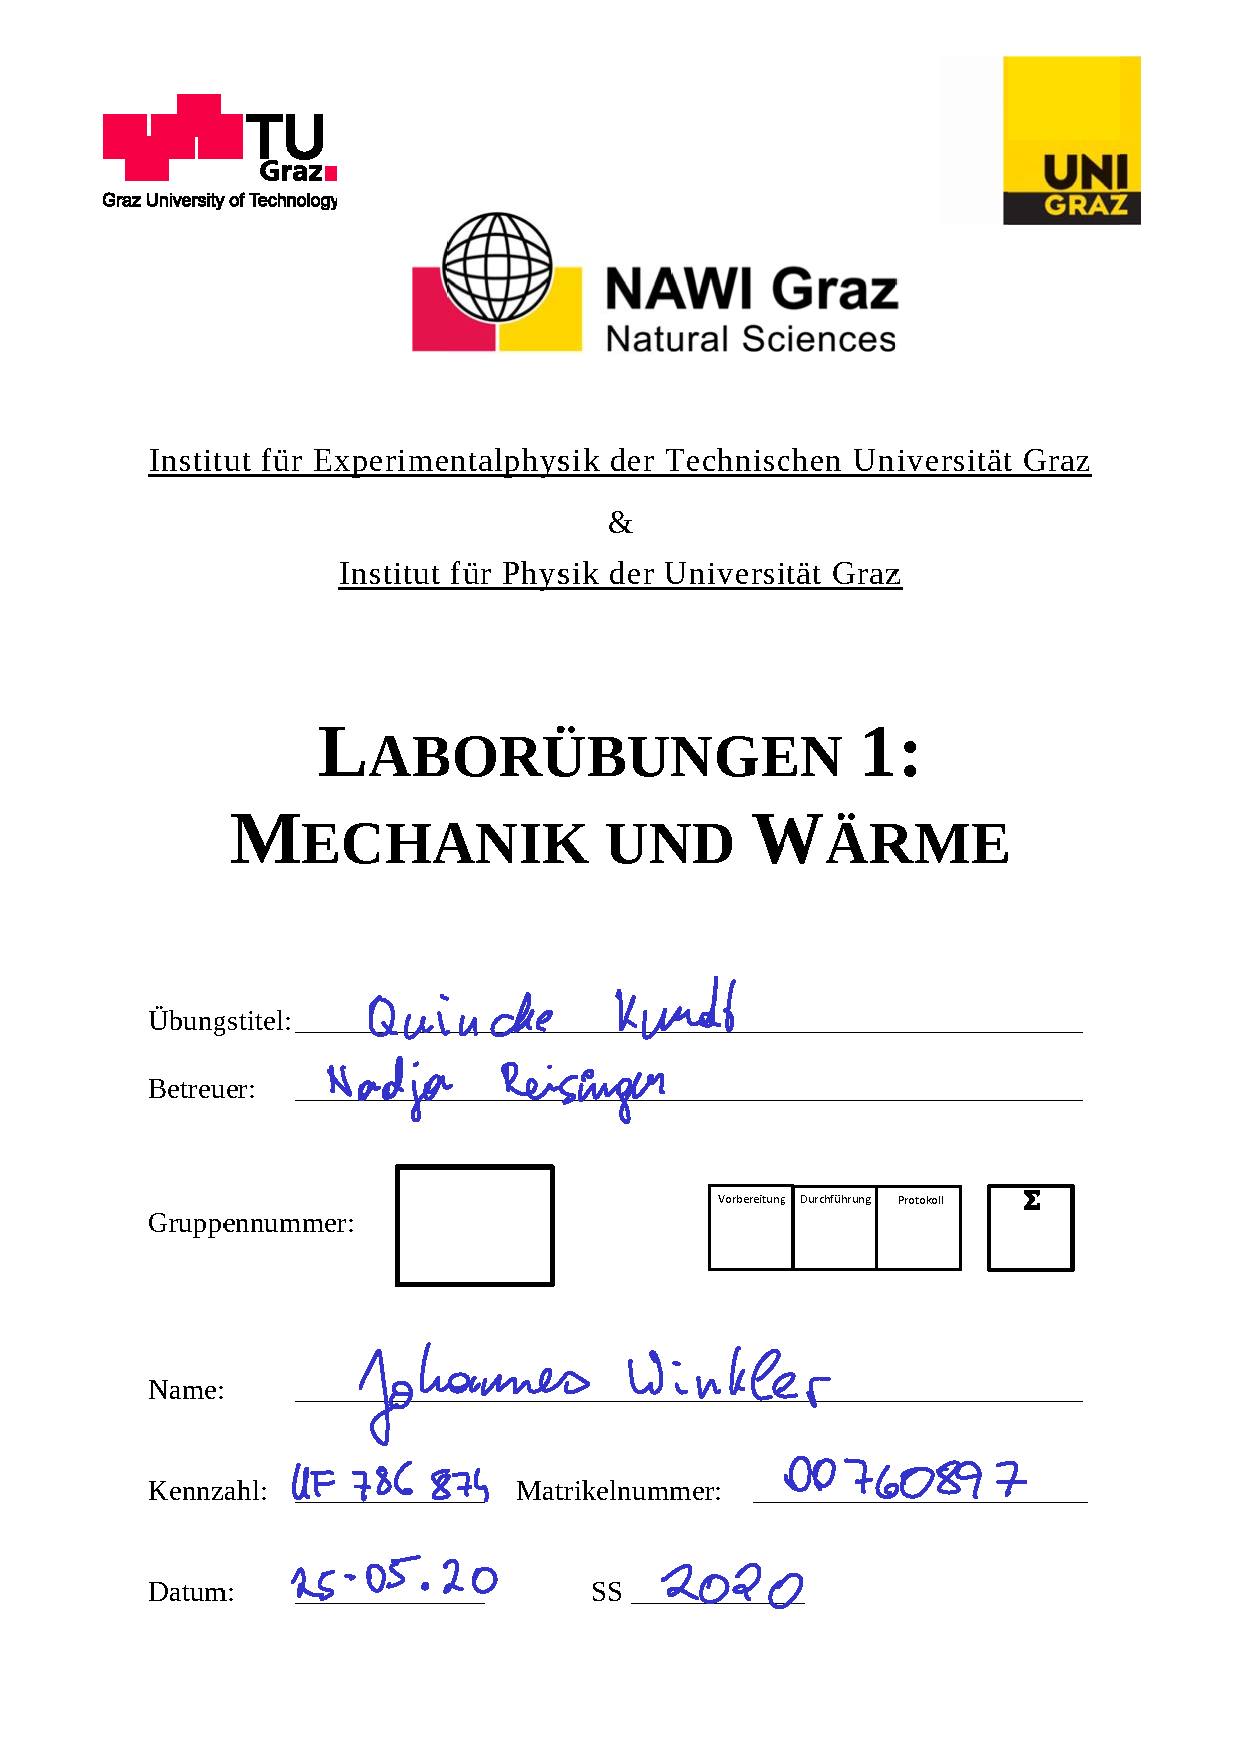
\includepdf[page=-]{deckblatt.pdf} 
 
 
\pagestyle{fancy}


\tableofcontents

\newpage


\section{Aufgabenstellung}
\begin{enumerate}
\item Bestimmung der Schwingungsknoten der stehenden Welle im Quincke-Resonanzrohr.
\item Bestimmung der Schallgeschwindigkeit in Luft.
\item Berechnung des Adiabatenexponenten von Luft.
\item Bestimmung der Wellenlänge einer stehenden Welle (5 Messungen) im Kundt'schen Rohr.
\item Berechnung des Elastizizätsmoduls des Stabes unter Verwendung der mit dem Quincke-Resonanzrohr bestimmten Schallgeschwindigkeit in Luft.
\end{enumerate}



\section{Grundlagen}
Der Schall breitet sich in Gasen als longitudinale Welle aus, d.h. die Teilchen schwingen in
Ausbreitungsrichtung der Welle. In zwei Medien gilt mit $\nu$ der Frequenz, mit $\lambda$, $\lambda^\prime$ und $c$, $c^\prime$ den jeweiligen Wellenlängen und Schallgeschwindigkeiten:
\begin{align}
\label{eq:clambda}
c = \lambda\cdot \nu \qquad \text{oder} \qquad c^\prime = \lambda^\prime\cdot \nu
\end{align}

Wird Schall reflektiert, so bilden, bei geeigneten Bedingungen, die mit der einfallenden interferierende reflektierte Welle eine stehende Welle. Für Reflexion an einem offenen Ende und am anderen starren Ende (Wasseroberfläche) gilt die Resonanzbedingung, dass die Länge der Luftsäule ein ungeradzahliges Vielfaches eines Viertels der Wellenlänge sein muss.
\begin{align}
l_1 = \frac14\cdot \lambda,~ l_2 = \frac34\cdot \lambda,~ l_3 = \frac54\cdot \lambda, \dots , l_n = \frac{2\cdot n-1}{4}\cdot \lambda, \qquad n=1,2,3,\dots
\end{align}

Der temperaturabhängige Quotient des Drucks $p$ und der Dichte $\rho$ steht mit $p_0$ (1013 mbar)
und $\rho_0$ ($1.29 \times 10^{-3}~$g/cm${}^3$ ), dem Luftdruck und -dichte bei $0^\circ$C auf Meereshöhe, und $\alpha$ dem Spannungskoeffizienten der Luft ($\alpha = 1/273.15~$K${}^{-1}$) im Zusammenhang:
\begin{align}
\frac{p}{\rho} = \frac{p_0}{\rho_0}\cdot (1 + \alpha\cdot\vartheta)
\end{align}
Damit ergibt sich aus der Schallgeschwindigkeit $c$ nach Laplace für die von der temperaturabhängige Schallgeschwindigkeit $c_T$:
\begin{align}
\label{eq:adiabatenindex}
c = \sqrt{\frac{p\cdot \kappa}{\rho}} \qquad \Rightarrow c_T = \sqrt{\frac{p_0\cdot \kappa\cdot (1 +\alpha\cdot \vartheta)}{\rho_0}}
\end{align}

Für Luft gilt näherungsweise im Temperaturbereich $-20~^\circ$C $\Rightarrow$ $40~^\circ$C die Zahlenwertgleichung:
\begin{align}
c[\text{m/s}] = 331.5 + 0.6\cdot\vartheta[{}~^\circ\text{C}]
\end{align}

Beim Übergang von einem Medium ins andere gibt sich nach Gl. \eqref{eq:clambda}
\begin{align}
\label{eq:clambda2}
\frac{c}{c^\prime} = \frac{\lambda}{\lambda^\prime}
\end{align}

d.h. in zwei verschiedenen Medien verhalten sich die Ausbreitungsgeschwindigkeiten einer Welle wie ihre Wellenlängen. Die Frequenz ändert sich dabei nicht. Wird also die Wellenlänge in beiden Medien gemessen, und ist die Schallgeschwindigkeit in einem Medium bekannt, so ist die Schallgeschwindigkeit im anderen Medium aus Gl. \eqref{eq:clambda2} bestimmbar.
Bei bekannter Dichte des Stabmaterials (Dichte von Glas bei Raumtemperatur: $\rho = 2500~$kg/m${}^3$)
kann sein Elastizitätsmodul $E$ aus der Gleichung für die Schallgeschwindigkeit bestimmt werden.
\begin{align}
\label{eq:figemodul}
c_{\text{Glas}} = \sqrt{\frac{E}{\rho}}
\end{align}

\section{Versuchsaufbauten}


\begin{figure}[H]
\caption{Das Quincke-Resonanzrohr. $F$ Frequenzgeber (1600 Hz), $R$ Glasrohr mit veränderbarem Wasserspiegel, AB Ausgleichsbehälter, $l$ Länge der Luftsäule, $\lambda$ Wellenlänge.}
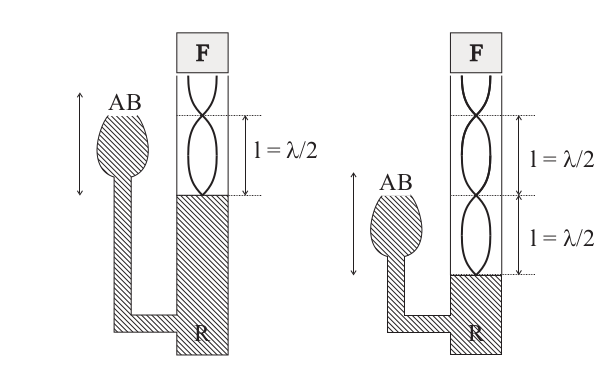
\includegraphics[height=5cm]{pic1.png}
\label{fig:resonanzrohr}
\end{figure}


\begin{figure}[H]
\caption{Die Kundt'sches Rohr. $\lambda_\text{Glas}$ , $\lambda_\text{Luft}$ Wellenlänge im longitudinal schwingenden Glasstab resp. in Luft.}
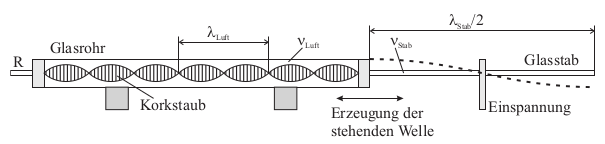
\includegraphics[width=\textwidth]{pic2.png}
\label{fig:rohr}
\end{figure}




\begin{figure}[H]
\caption{Bestimmung der Wellenlänge.}
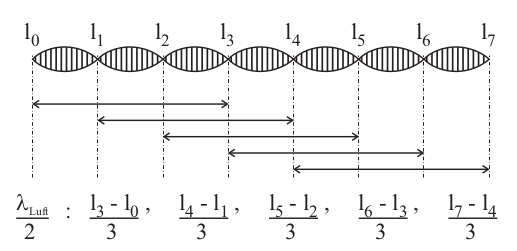
\includegraphics[width=\textwidth]{pic3.png}
\label{fig:wellenlaenge}
\end{figure}


Zu Abb. \ref{fig:resonanzrohr} Das Resonanzrohr ist ein Glasrohr, das eine Luftsäule veränderbarer Länge enthält. Durch Heben und Senken des Ausgleichsbehälters kann man die Länge der Luftsäule variieren. Die Luftsäule wird durch einen Schallgeber über der Öffnung des Rohres zum Schwingen an-
geregt. Die Frequenz ist durch den Schallgeber vorgegeben. Die Wellen laufen bis zum Ende
der Luftsäule (Wasseroberfläche), werden dort reflektiert, und interferieren mit den einfallenden
Wellen, so daß sich im Rohr eine stehende Welle ausbildet. Ist die Luftsäule so lang, daß sich an
der Wasseroberfläche ein Schwingungsknoten, an der Rohröffnung aber ein Schwingungsbauch
befindet, so besteht Resonanz zwischen dem Frequenzgeber und der Luftsäule im Rohr.

Zu Abb. \ref{fig:rohr}: Die vom Stabende bei longitudinaler Anregung ausgehende Schallwelle pflanzt sich in das Glasrohr fort, und wird am Ende des Glasrohres reflektiert. Es entsteht eine stehende
Welle, die mittels Korkpulver in der Röhre sichtbar gemacht wird. Die stehende Welle bildet
sich nur dann scharf aus, wenn am geschlossenen Ende des Rohres ein Wellenknoten liegt. Dies
wird erreicht, indem man die Länge der Luftsäule durch Verschieben des Glasrohres variiert.


Zu Abb. \ref{fig:wellenlaenge}: Zur Bestimmung der Wellenlänge in Luft $\lambda$ Luft werden zunächst alle Knotenstellen ausgemessen $(l_0, l_1, \dots, l_n)$. Soll zur Verbesserung der Ablesefehler der Knotenstellen die größtmögliche Anzahl von Messungen zur Mittelwertbildung verwendet werden, so werden als
Anfangs- und Endknotenstellen die Knoten herangezogen, deren Abstand voneinander gerade größer ist als $a$/2, wobei $a$ der Abstand zwischen dem ersten und dem letzten zur Messung geeigneten Knoten ist. Wie aus Abb. \ref{fig:wellenlaenge} ersichtlich, ergeben sich dadurch beispielsweise für 6 Messpunkte 3 voneinander unabhängige Mittelwerte für $\lambda_\text{Luft}/2$.

\newpage

\section{Geräteliste}


Da aufgrund der Corona-Situation keine physikalische Anwesenheit im Labor möglich ist, kann ich auch die genauen Serien- und Gerätenummern angeben.

Da auch die Gebrauchsanleitung und Datenblätter der Werkzeuge nicht vorhanden sind, werden die Messfehler dieser Geräte geschätzt.


\begin{table}[h]
\caption{Geräteliste}

\begin{tabular}{llll}
Gerät  & Bezeichnung/Nr. & Hersteller & Genauigkeit \\
\hline
Quincke Resonanzrohr & axxxx \\
Lautsprecher & bxxxx \\
Thermometer & GTH 1170 & Gresinger &  \\
Flüssigkeitsgefäß & dxxxx \\
Lineal & exxxx  & & $\Delta l = 1~$mm \\
Barometer & fxxxx \\
Kundt'sches Rohr & gxxxx \\
Trillerpfeife & hxxxx\\
Piezosensor & kxxxx\\
Stab aus Stahl & ... \\
Stab aus Messing & ... \\
Stab aus Aluminium & ... \\
Stab aus Kupfer & ... 
\end{tabular}
\end{table}

\newpage
\section{Versuchsdurchführung und Messergebnisse}


\subsection{Quincke Resonanzrohr}

Zuerst wird im Quincke Resonanzrohr ein Ton mit einer Frequenz von 1600~Hz eingespielt. Die Raumtemperatur beträgt $18.4~^\circ$C. Der Wasserstand im Quincke Rohr wird immer solange variiert, bis der Ton laut zu hören ist. An diesen Stellen kommt es zu einer Überlagerung. Die Höhendifferenz zweier solcher benachbarten Stellen ist die halbe Wellenlänge. Im ersten Versuch messen wir diese Höhen, um daraus die Wellenlänge $\lambda$ abschätzen zu können. Die Messwerte sind in Tabelle~\ref{tab:quincke_rohr}.

\begin{table}[H]
\caption{Messung der Wellenlänge mit Quincke-Resonanzrohr. Die Zeilen sind die Messreihen, die Spalten sind jene gemessenen Höhen $l_i$ der Flüssigkeit, sodass man den Ton laut hört. Die Messunsicherheit der Längen ist mit $\Delta l = 1~$mm spezifiert.}
\label{tab:quincke_rohr}
\begin{tabular}{l|rrrrr}
Messung Nr & $l_1$ / cm & $l_2$ / cm  &  $l_3$ / cm  &  $l_4$ / cm  & $l_5$ / cm  \\
\hline
1 & 14.0 &     25.0 &  			36.0 & 		46.5 &  	56.5 \\
2 & 14.5 &     25.0 &  		  	36.0 &		46.0 &  56.0 \\
3 & 14.0 & 		24.5 &     		35.0 &		46.0 &  56.5 \\
4 & 14.5 & 		25.0 &	   		36.0 &  		46.0 &  57.0 \\
5 & 14.0 &  	25.5 &  			36.0 &		46.5 &  57.5 
\end{tabular}
\end{table}
Die Differenz zwischen zwei übereinander stehenden Werten liefert jeweils eine Näherung für $\lambda/2$. Im Mittel erhält man insgesamt $\frac{\lambda}{2} = 10.625$~cm, oder anders geschrieben $\lambda = 21.25$~cm.



\subsection{Kundt'sches Rohr}

Beim Kundt'schen Rohr ist zuerst die Tonhöhe einer Trillerpfeife zu bestimmen. Hierbei wird mit dieser in ein Glasrohr gepfiffen, in der sich Korkstaub. Die Messwerte sind in Tabelle~\ref{tab:rohr}

\begin{table}[H]
\caption{Messwerte bei der Wellenlängenmessung der Trillerpfeife mit Hilfe des Kundt'schen Rohrs. Die Unsicherheit bei Längenmessungen ist $\Delta l = 1~$mm.}
\label{tab:rohr}
\begin{tabular}{l|llllll}
Messung Nr &  $l_1$ / cm &  $l_2$ / cm &  $l_3$ / cm &  $l_4$ / cm &  $l_5$ / cm &   $l_6$ / cm \\
\hline
1 & 46.0 & 52.0 & 58.0 & 63.0 & 69.0 & 73.5 \\
2 & 46.0 & 52.0 & 57.5 & 62.5 & 67.5 & 73.0
\end{tabular}

\end{table} 
Die Differenz zwischen Minimum und Maximum geteilt durch 5 ergibt eine mittlere halbe Wellenlänge. Über beide Messreihen gemittelt ergibt das insgesamt $\lambda/2 = 5.45$~cm, was $\lambda = 10.9$~cm entspricht.




\begin{table}[H]
\caption{Messwerte bei der Wellenlängenmessung im Glasrohr.}
\begin{tabular}{l|llllll}
Messung Nr & $l_1$ / cm & $l_2$ / cm & $l_3$ / cm & $l_4$ / cm & $l_5$ / cm &  $l_6$ / cm \\
\hline
1 & 42 & 52 & 63 & 72 & 82 & 93 \\
2 & 42 & 52 & 62 & 73 & 82 & 92
\end{tabular}
\end{table} 

Die Differenz von Minimum und Maximum geteilt durch 5 ergibt wieder die mittlere halbe Wellenlänge. Auf beide Messreihen gemittelt ergibt sich $\lambda/2 = 10.1$~cm und daher ist $\lambda=20.2$~cm.



\subsection{Schallgeschwindigkeit in Festkörpern}

Um die Schallgeschwindigkeit in den Materialien Messing, Aluminium, Kupfer und Stahl zu bestimmen, werden 4 an Stäben aus dem jeweiligen Material an einer Seite eine Schwingung durch Klopfen erzeugt, und an der jeweils anderen Seite gemessen. Die Schallwelle wird an einem Ende des Stabes reflektiert, sodass zwischen den messbaren Schallwellen jeweils die doppelte Länge des Stabes zurückgelegt wird. Jeder Stab ist $\ell=1.5$~m lang mit einer Unsicherheit $\Delta ell = 1~$mm.

Die Schallenwellen an einem Endpunkt des Stabes wird mit einem Piezo-Sensor aufgezeichnet. So erhält man eine periodisch wiederkehrende Schallwelle. Zwischen je zwei Maxima der Schallwelle kann man die Zeit bestimmen, die eine Schallwelle für die Länge $2\cdot \ell = 3$~m benötigt, wobei sich hier die Unsicherheit ebenfalls verdoppelt. Für jedes Material wird 10 mal gemessen. Für jedes Material und für jede Messung wird über die Abstände zwischen den Maximas gemittelt und in Tabelle \ref{tab:schall} dargestellt. Gemittelt wurde wie in Kapitel 3 besprochen.

\begin{table}[H]
\caption{Messwerte für die Schallgeschwindigkeit in Festkörpern. Wurde am Computer ausgewertet. Alle Zeiten $t_i$ sind in Millisekunden angegeben, was aus Platzgründen in der Tabelle nicht erwähnt wird.}
\label{tab:schall}

\begin{tabular}{l|llllllllll|l}
& $t_1$ & $t_2$  & $t_3$ & $t_4$ & $t_5$  & $t_6$ & $t_7$  & $t_8$ & $t_9$ & $t_{10}$ & $\overline{t}$ \\
\hline
Messing    & 0.80 & 0.80 & 0.85 & 0.85 & 0.80 & 0.85 & 0.85 & 0.85 & 0.80 & 0.80 & 0.825\\
Aluminium  & 0.55 & 0.60 & 0.60 & 0.55 & 0.60 & 0.55 & 0.60 & 0.65 & 0.60 & 0.55 & 0.585\\
Kupfer     & 0.80 & 0.80 & 0.80 & 0.80 & 0.80 & 0.80 & 0.80 & 0.85 & 0.80 & 0.80 & 0.805\\
Stahl      & 0.60 & 0.60 & 0.60 & 0.60 & 0.60 & 0.65 & 0.60 & 0.60 & 0.60 & 0.60 & 0.605
\end{tabular}
\end{table}



\newpage
\section{Auswertung}

\subsection{Bestimmung der Schallgeschwindigkeit in Luft}

Aus Formel \eqref{eq:clambda} kann man die Schallgeschwindigkeit berechnen, also 
\begin{align}
c = \lambda\cdot \nu = 0.2125 \cdot 1600 = 340~\text{m s}^{-1}
\end{align}
Deren Unsicherheit ist durch die Größtfehlermethode gegeben als
\begin{align}
\Delta c &= \left|\frac{\partial c}{\partial \lambda}\right| \cdot \Delta \lambda + \left| \frac{\partial c}{\partial \nu}\right| \cdot \Delta \nu = \Delta\lambda\cdot \nu + \lambda\cdot \Delta \nu \\
&= 0.001\cdot 1600 + 0.2125\cdot 0.01 = 1.6~\text{m s}^{-1}
\end{align}
Die Frequenz ist im Video mit $\nu=1600~$Hz gegeben mit einer Unsicherheit von $\Delta\nu=0.01~$Hz. Für die Wellenlänge nehmen wir den Mittelwert für die Wellenlängen, die man durch Differenzbildung aus Tabelle \ref{tab:quincke_rohr} ablesen kann.

Zusammenfassend erhält man für die Schallgeschwindigkeit folgendes Messergebnis:
\begin{align*}
c = (340.0 \pm 1.6)~\text{m s}^{-1}
\end{align*}

\subsection{Bestimmung des Adiabatenindex von Luft}

Zuerst benötigt man den Druck auf der angegebenen Höhe. Durch das Barometer bekommt man den virtuellen Druck, der auf Meereshöhe herrschen würde. Dieser ist $p_M = 1008$~hPa. Durch die Barometrische Höhenformel (vgl. \cite{demtr1}) ergibt sich für den Druck
\begin{align}
p_0 = p_M\cdot \exp(-\rho_0 \cdot g \cdot h / p_M) \approx 96430.36~\text{Pa}
\end{align}
Zahlmäßig ist die Dichte der Luft mit $\rho_0 = 1.29~$kg/m${}^3$ gegeben. Zusätzlich weiß man aus \cite{graz}, dass die Stadt Graz auf einer Höhe von Näherungsweise $h=353$~m liegt.

Aus Formel \eqref{eq:adiabatenindex} folgt für den Adiabatenindex
\begin{align}
\kappa = \frac{c_T^2\cdot \rho_0}{p_0\cdot (1 + \alpha\cdot \vartheta)} = 1.449
\end{align}
Wichtig ist, dass $\vartheta$ in Grad Celsius in diese Gleichung eingesetzt wird, und nicht in Kelvin.

Wir berechnen nun die Unsicherheit
\begin{align}
\Delta\kappa &= \left| \frac{\partial\kappa}{\partial c_T} \right| \cdot \Delta c_T + \left| \frac{\partial\kappa}{\partial \vartheta} \right| \cdot \Delta \vartheta + \left| \frac{\partial\kappa}{\partial p_0} \right| \cdot \Delta p_0 \\
\Delta\kappa &= \frac{2\cdot c_T  \cdot \Delta c_T \cdot \rho_0}{p_0\cdot (1 + \alpha\cdot \vartheta)} + \frac{c_T^2\cdot \rho_0\cdot \alpha \cdot \Delta \vartheta}{p_0\cdot (1 + \alpha\cdot \vartheta)^2} + \frac{c_T^2\cdot \rho_0 \cdot \Delta p_0}{p_0^2\cdot (1 + \alpha\cdot \vartheta)} \\
\Delta \kappa &= \frac{c_T\cdot \rho_0}{p_0\cdot (1+\alpha\cdot \vartheta)}\cdot \left(2\cdot \Delta c_T +  \frac{c_T\cdot \alpha\cdot\Delta\vartheta}{(1+\alpha\cdot \vartheta)} + \frac{c_T\cdot \Delta p_0}{p_0}\right)
\end{align}
Wir setzen $\Delta c_T = 1.6~$m~s${}^{-1}$ (wie bereits berechnet). Zusätzlich sei $\Delta\vartheta = 0.1~^\circ$C und $\Delta p_0 = 20~$Pa. Dann ergibt sich für die Unsicherheit
\begin{align*}
\Delta \kappa = 0.015
\end{align*}

Insgesamt ergibt sich also
\begin{align*}
\kappa = (1.449 \pm 0.015)
\end{align*}

\subsection{Bestimmung der Frequenz der Trillerpfeife}

Die Schallgeschwindigkeit $c = 340$~m~s${}^{-1}$ wurde bereits gemessen. Für die Wellenlänge der ergab die Messung $\lambda=0.109$~m.
Es folgt nun
\begin{align}
\nu = \frac{c}{\lambda} = 3119.27~\text{Hz}
\end{align}
Die Unsicherheit der Frequenz ist
\begin{align}
\Delta\nu &= \left|\frac{\partial \nu}{\partial c}\right| \cdot \Delta c + \left|\frac{\partial \nu}{\partial c}\right| \cdot \Delta c \\
&= \frac{\Delta c}{\lambda} + \frac{c\cdot \Delta\lambda}{\lambda^2} 
\end{align}
wobei $c$ und $\Delta c$ bereits bestimmt wurde. Wenn für $\Delta\lambda=1$~mm angenommen wird, dann erhält man für die Unsicherheit 
\begin{align}
\Delta \nu = \frac{1.6}{0.109} + \frac{340 \cdot 0.001}{0.109^2} = 43.32~\text{Hz}
\end{align}
Die Frequenz der Trillerpfeife beträgt also
\begin{align*}
\nu = (3119.27\pm 43.32)~\text{Hz}
\end{align*}
\subsection{Bestimmung der Schallgeschwindigkeit und des Elastizitätsmoduls von Glas}

Die Dichte von Glas ist beim Versuch gegeben mit $\rho=2500$~kg/m${}^3$. Zusätzlich wissen wir, dass $\lambda_\text{Glas} = 3$~m sind, während $\lambda_\text{Luft} = 20.2$~cm beim Versuch gemessen wurden. Aus Gleichung \eqref{eq:clambda2} erhält man
\begin{align}
c_\text{Glas} &= \frac{\lambda_{\text{Glas}}}{\lambda_\text{Luft}} \cdot c_\text{Luft} \\
c_\text{Glas} &= \frac{3}{0.202}\cdot 340 = 5050~\text{m s}^{-1}
\end{align}

Der Elastizitätsmodul lässt sich aus Gleichung \eqref{eq:figemodul} bestimmen. Er ist
\begin{align}
\label{eq:emodulglass}
E_\text{Glas} &= c_\text{Glas}^2 \cdot \rho \\
&= 64~\text{GPa}
\end{align}

Die Unsicherheiten lassen sich folgend ausdrücken
\begin{align}
\Delta c_\text{Glas} &= \left| \frac{\partial c_\text{Glas}}{\partial \lambda_\text{Glas}} \right| \cdot \Delta \lambda_\text{Glas} + \left| \frac{\partial c_\text{Glas}}{\partial \lambda_\text{Luft}} \right| \cdot \Delta \lambda_\text{Luft} + \left| \frac{\partial c_\text{Glas}}{\partial c_\text{Luft}} \right| \cdot \Delta c_\text{Luft} \\
&= \frac{\Delta \lambda_{\text{Glas}}}{\lambda_\text{Luft}} \cdot c_\text{Luft} + \frac{\lambda_{\text{Glas}}}{\lambda_\text{Luft}^2} \cdot c_\text{Luft}\cdot \Delta\lambda_\text{Luft} + \frac{\lambda_{\text{Glas}}}{\lambda_\text{Luft}} \cdot \Delta c_\text{Luft} \\ 
&= \frac{0.001}{0.202}\cdot 340 + \frac{3}{0.202^2}\cdot 340\cdot 0.001 + \frac{3}{0.202}\cdot 1.6 \\
&= 50.4743~\text{m s}^{-1}
\end{align}
wobei wir Längenmessungen wieder auf einen Fehler von $\pm 1$~mm annehmen. 

\begin{align}
\label{eq:emodulglass2}
\Delta E_\text{Glas} &= \left| \frac{\partial E_\text{Glas}}{\partial c_\text{Glas}}\right| \cdot \Delta c_\text{Glas} = 2\cdot c_\text{Glas}\cdot \Delta c_\text{Glas}\cdot \rho = 1.3~\text{GPa}
\end{align}


\subsection{Schallgeschwindigkeit in Festkörpern}

In diesem Fall wird die Schallgeschwindigkeit durch Weg pro Zeit bestimmt. Der Weg ist in unserem Fall $\ell=3~$m, wobei die Unsicherheit für die Weglänge laut Video $2$~mm ist. Durch die Verdoppelung des Weges wären es insgesamt $\Delta\ell=4$~mm. Für das Ablesen der Zeit nehmen wir eine Unsicherheit von $\Delta t = 10^{-4}$~s an.

Die Schallgeschwindigkeit und deren Unsicherheit sind daher
\begin{align}
c &= \frac{\ell}{t} \\
\Delta c &= \left| \frac{\partial c}{\partial\ell}\right| \cdot \Delta \ell + \left|\frac{\partial c}{\partial t}\right| \cdot \Delta t = \frac{\Delta \ell}{t} + \frac{\ell}{t^2}\cdot \Delta t \\
&= \frac{0.004}{t} + \frac{0.0003}{t^2}
\end{align}
Ähnlich zu Gleichungen \eqref{eq:emodulglass} und  \eqref{eq:emodulglass2} erhalten wir den Elastizitätsmodul und dessen Unsicherheit 
\begin{align}
E &= c^2\cdot \rho \\
\Delta E &= 2\cdot c\cdot \Delta c\cdot \rho
\end{align}
Die Dichte wird als gegeben und konstant angenommen. In \cite{giancoli} findet man
\begin{align}
\rho_\text{Stahl} &= 7800~\text{kg~m}^{-3} \\
\rho_\text{Aluminium} &= 2700~\text{kg~m}^{-3} 
\\
\rho_\text{Kupfer} &= 8900~\text{kg~m}^{-3} 
\end{align}
Die Dichte von Messing ist abhängig von der genauen Zusammensetzung (siehe \cite{messing}), als Mittelwert können wir aber 
\begin{align}
\rho_\text{Messing} &= 8635~\text{kg~m}^{-3} 
\end{align}
annehmen. Die ausgerechneten Werte finden sich im nächsten Kapitel.


\section{Zusammenfassung und Diskussion}


Das Messergebnis für die Schallgeschwindigkeit beträgt
\begin{align*}
c = (340.0 \pm 1.6)~\text{m s}^{-1}
\end{align*}
Gemäß \cite{demtr1}, Abschnitt 11.9.5.5. bzw Tabelle 11.3 passt dieses Ergebnis unter Berücksichtigung der Unsicherheiten zu den in der Literatur vorhandenen Angaben.

Der Adiabatenindex ist
\begin{align*}
\kappa = (1.449 \pm 0.015)
\end{align*}
Gemäß der Quelle \cite{exponent} liegt der Adjabatenkoeffizient für trockene Luft bei $0~^\circ$C bei ca 1.4. Unser Wert stimmt zwar von der Größenordnung, jedoch liegt der Wert aus dieser Quelle außerhalb der Unsicherheit. Daher ist davon auszugehen, dass unsere Messfehler größer sind als angenommen.

Die Frequenz der Trillerpfeife ist
\begin{align*}
\nu = (3119.27\pm 43.32)~\text{Hz}
\end{align*}

Für Schallgeschwindigkeit und Elastizitätsmodul von Glas ergeben sich
\begin{align*}
c_\text{Glas} &= (5050 \pm 50)~\text{m s}^{-1} \\
E_\text{Glas} &= (63 \pm 1.3)~\text{GPa}
\end{align*}

Für die Festkörper ergibt sich
\begin{align*}
c_\text{Messing} &= (3636 \pm 446)~\text{m s}^{-1} \\
E_\text{Messing} &= (114 \pm 28)~\text{GPa} \\
c_\text{Aluminium} &= (5128 \pm 883)~\text{m s}^{-1} \\
E_\text{Aluminium} &= (71 \pm 24)~\text{GPa} \\
c_\text{Kupfer} &= (3727 \pm 468)~\text{m s}^{-1} \\
E_\text{Kupfer} &= (124 \pm 31)~\text{GPa} \\
c_\text{Stahl} &= (4959 \pm 826)~\text{m s}^{-1} \\
E_\text{Stahl} &= (192 \pm 64)~\text{GPa}
\end{align*}
Diese Werte für den Elastizitätsmodul entsprechen mit den jeweiligen Unsicherheiten den Werten der Quelle \cite{emodul}. Jener von Messing liegt zwischen 102 und 125 GPa, jener von Aluminium bei 69 GPa, bei Kupfer bei 117 und bei Stahl sind die Werte 180 und 200 angegeben, die beide innerhalb der Unsicherheit liegen. Ähnlich verhält es sich bei den Schallgeschwindigkeiten, wie sie in \cite{schall} und \cite{schall2} nachgelesen werden können.

\subsection{Die Frage zur Schallgeschwindigkeit im Wasser}

Für die Bestimmung der Schallgeschwindigkeit im Wasser wird ein Boot, eine Glocke, ein Lichtblitz, und eine Hörmuschel benötigt. Die Lichtgeschwindigkeit ist als bekannt vorausgesetzt. Nun kann man am Ufer die Glocke und die Hörmuschel vom Boot aus in einer definierten Entfernung zum Ufer ins Wasser tauchen. Wenn die Glocke klingt, dann gibt jene Person im Boot per Licht eine Benachrichtigung, sobald der Schall angekommen ist.

Die Person, welche den Schall verursacht hat, kann dann die Zeit zwischen Ursprung des Schalls und Lichtsignal messen. Durch die definierte Länge ergibt sich die Geschwindigkeit.


\begin{thebibliography}{9}
\bibitem{demtr1} W. Demtröder, \emph{Experimentalphysik 1: Mechanik und Wärme}, Springer-Spektrum, 8. Auflage, 2018.

\bibitem{giancoli} D. Giancoli, \emph{Physik}, Pearson, 4. Auflage, 2019.

\bibitem{graz} \url{https://www.graz.at/cms/beitrag/10034466/7772565/Zahlen_Fakten_Bevoelkerung_Bezirke_Wirtschaft.html} (Stand: \today)

\bibitem{exponent} \url{https://webbook.nist.gov/chemistry/fluid/} (Stand: \today)

\bibitem{messing} \url{https://de.wikipedia.org/wiki/Messing} (Stand: \today)

\bibitem{schall} \url{https://de.wikipedia.org/wiki/Schallgeschwindigkeit} (Stand: \today)

\bibitem{schall2} Joseph L. Rose: Ultrasonic Waves in Solid Media. Cambridge University Press, 2004.

\bibitem{emodul} \url{https://www.engineeringtoolbox.com/young-modulus-d_417.html} (Stand: \today)
\end{thebibliography}

\end{document}
